\chapter{Design and Specification}\label{ch_method}

This chapter details the design decisions for ``Urban Explorer'' (the
app produced as part of this project) and how we use gamification in
``Urban Explorer'' to achieve the goals of the project. Core elements
of the project are formally defined and important implementation
details are also discussed.

\section{Design Aims}

The idea of the game is to travel around the world without physically
having to be there, inviting the user to realise the scale of the
world whilst gaining the positive benefits of outdoor exercise. A user
may decide to run around areas in Scotland (the Scotland Mission) and
this is achieved through routes such as Glasgow to Edinburgh. Each
route is further broken up into manageable stages of a few kilometres
and users are awarded badges based on stages/routes completed and
overall distance and time. This hierarchy of goals gives a natural
progression of success.

We intend to examine whether or not this type of encouragement
has potential to work with outdoor exercise. Metrics will be tracked
for individual users to monitor their exercise duration and frequency
and will be used to encourage that user to exercise. These metrics will
then be used to form the basis of our conclusion.

The design aims of the project are then as follows:
\begin{enumerate}
  \item To provide incentives that become intrinsically
    rewarding. Rewards are primarily linked to stage and route 
    completion and these accumulate to the completion of the entire
    mission - every achievement brings the user closer to a larger
    success. 
  \item To provide long and short term goals to fulfil the sense of
    achievement. The long term goals are Route completion and these are
    fulfilled by the easily achievable short term goals of Stages -
    for example the Central Park Route contains four stages, one for
    each edge of the park and these stages are easily achievable in an
    exercise session.
    \begin{enumerate}
      \item Stage completion - unlock a photograph of the stage or of
        a key landmark near the stage. 
      \item Route Completion - a gold, silver or bronze medal is
        awarded for completing a route in a given time period. A route
        is completed when all the stages in a route are completed.
    \end{enumerate}
\end{enumerate}

\section{Defining Gamification in this Application}

Previously we noted the definition of gamification by
\citet{gamification_book} as ``The process of
game-thinking and game mechanics to engage users and solve
problems.''. To fulfil this definition we must define what we mean
by: \emph{game-thinking}, \emph{game mechanics}, \emph{users} and
\emph{problems}. 

In our context the \emph{problem} is that the there is the perception
that there is a ``lack of time to take exercise''\cite{exercise}, a
problem which has been statistically reduced in later reports by
redefining what an allowed exercise duration
is\cite{exercise_2012}. The later report indicated that exercise
sessions of 10 minutes or more are valid,  which our application
accommodates for. 

The \emph{users} that we are targeting are those who have the
potential to capitalise on their everyday travels to either extend
these journeys or travel with more vigour. This was explored in Section
\ref{sec:targeted_users}.  

\emph{Game mechanics} are the elements we add to a process or
interaction to change the context of the process to encourage
and change behaviour. We do this through creating a \emph{story} that
a user can \emph{``Run Around the World''} by completing
routes. There is a progression model involved whereby completing one
route unlocks the next. The progression model is a \emph{mechanic}
which gives users direction through the game. By allowing each route
to be unlocked by completing a previous one we create explicit goals
that the user can aim for. A route is composed of several stages which
you complete as you progress along the route, completing each of these
stages unlocks a picture for that stage. This is a \emph{reward} that
the user will achieve simply by playing the game. The user will also
receive a medal (\emph{reward}) if they complete an entire route
within a given time. Both of these \emph{reward} metrics will
encourage the user in different ways: although both metrics are
extrinsic in nature, the picture unlocks are solely indicators of
success whereas the medals are indicators of the user excelling at the
task. The picture unlocks are added motivation for the user to achieve
a better medal for a specific route.

Finally, \emph{game-thinking} is the definition of the users
objectives to try to understand how they will find success. It can
also be the process used to explore what the users perception of the
interaction is. In a standard game context the user wishes to maximise
the likelihood that they will win or succeed. The user knows they have
won when they complete a route in a fast enough time to achieve
the best medal. A user can also succeed by completing the stages that
make up a given route, which unlocks the pictures for each
stage. Therefore the only way to succeed in either case is to
exercise, so our \emph{goals} help us solve our initial
\emph{problem}. 

The context of our application of gamification is exercise, but if we
can coerce the users into focusing on the game instead of the exercise
then our motivation becomes \emph{intrinsic} as the user wants to
achieve the goals for personal satisfaction instead of using the goals
to justify exercise. A larger analysis of this idea is required to
determine if this can be achieved in this context. Existing games like
\emph{Zombies, Run!}(Section \ref{sec:zombies}) where there is a large
meta-game that surrounds the exercise activity do indicate that this
coercion may be possible, however the benefits are not understood and
a larger analysis will help to discover these benefits. 

\section{User Requirements}
From discussions in project meetings and within the authors peer
group, the following requirements were elicited. The initial
requirements were a subset of the following requirements but these
were expanded upon to the following set as the project progressed. The
\emph{MoSCoW} prioritisation \cite{moscow} of \textbf{M}ust Have,
\textbf{S}hould Have, \textbf{C}ould Have and \textbf{W}on't Have This
Time was used to categorise these requirements and can be shown in
Table \ref{table:moscow}. The status of each of these requirements is
also shown in this table.

\begin{table}[h]
  \centering
  \begin{threeparttable}[b]
  \begin{tabular}{ | c | p{12cm} | c | } \hline 
    Priority & Task & Completed \\\hline
    M & Device registration with server & \checkmark \\\hline
    M & Obtain location data from the device and transmit this data to
    the server & \checkmark \\\hline
    M & Determine the distance between to sets of location coordinates
    & \checkmark \\\hline
    M & Display all routes to the user and allow them to pick a route
    to exercise along & \checkmark \\\hline
    M & Display current progress along a route to a user & \checkmark
    \\\hline
    M & Display distance until next unlock (reward) & \checkmark
    \\\hline
    M & Show the user their current achievements and how to achieve
    their next one & \checkmark \\\hline
    M & Allow the user to start and end an exercise session &
    \checkmark \\\hline
    M & Update the session as a user progresses in an exercise session
    & \checkmark \\\hline
    M & Show the user the distance they have travelled and time they
    have spent exercising when in a session & \checkmark \\\hline
    S & Show the user the picture they will unlock by completing the
    stage they are currently on when in an exercise session &
    \checkmark \\\hline 
    S & Provide help information to the user on request & \checkmark
    \\\hline 
    S & Provide a notification when the user unlocks a picture
    (completing a stage or a route) or is awarded a medal & \\\hline 
    S & Store the last route a user exercised on to give the user a
    shortcut when the app launches to continuing their progress on
    this route & \\\hline
    C & Share results of exercise session to social media sites
    (Facebook and Twitter) & \\\hline
    C & Send push notifications\tnote{1} to the device for
    notification of success and to inform the user of new content &
    \\\hline
    W & Integrate with pedometer devices such as the Fitbit (Section
    \ref{sec:fitbit}) for more accurate distance monitoring &
    \\\hline
    W & Use the motion sensors on the phone with machine learning
    techniques to use the phone as a pedometer & \\\hline
  \end{tabular}
  \begin{tablenotes}
    \item[1] Android Push Notifications - \url{http://developer.android.com/google/gcm/index.html}
  \end{tablenotes}
  \caption{MoSCoW Requirements Prioritisation}
  \label{table:moscow}
  \end{threeparttable}
\end{table}

\section{Specification}
\label{sec:specification}
The implementation specifics of this project are defined below with
the overall development of the project shown in the following sections.
An overarching goal for this implementation is to minimise the end cost
for the user. This cost takes two forms: 
\begin{enumerate}
\item Time - Time taken to load and process content from the server.
\item Data - Network costs incurred through data transfer on mobile networks.
\end{enumerate}

Content, like the routes that a user can travel along or the
achievements they can be awarded, can either come packaged inside the
application or can be loaded from the server each time the app
launches. If the content is packaged inside the app then the overall
loading time of the app will be small but we will require an update to
the app every time we want to add or modify new content. The overall
size of the app on the phone will also be larger. By loading content
from the server once the app has launched we can allow new content to
be added easily. This approach does incur a longer loading time however.

We can mitigate further loading times by storing the response from the
server when we ask for content and refer to this local store
instead of contacting the server again. Referring to a local data
store is orders of magnitude faster than a network response time. This
process is called \emph{caching} and will also help to reduce the
\emph{data cost} of this application: by caching the data received we
remove the need to make that request again and so reduce the number of
network transfers. 

We must be able to identify a user so we can correctly track the
progress that a user makes. We can achieve this without requiring any
information that could identify the user outside the system by using a
unique device identifier provided by the phone. From a privacy 
perspective this means we have a fully anonymous system where we
cannot identify what person used each phone but we can still track
each user in a reliable way. A side effect of this decision is that
the device handles registration and log in as a background task which
allows the user to begin using the application almost immediately
without requiring any input or interaction from the user. Removing
this registration and log in barrier streamlines the interaction flow
of the application by removing the \emph{time cost} that a user would
incur should explicit registration or log in be required. This in turn
allows the user to begin exercising with the application immediately.

\subsection{Platform and Frameworks}
The mobile application is developed using PhoneGap \cite{phonegap}, 
a tool which allows you to develop a mobile app as if it were
a web app, and then package it as a mobile app. The decision to use
PhoneGap instead of building a native app is because of its rapid
development cycle, the option to deploy to multiple platforms easily
without changing the code base and the familiarity that the author has
with web technologies. Because of this, our application is written
using HTML, JavaScript, and CSS3. 

The Twitter Bootstrap CSS framework\cite{bootstrap} was used due to
the excellent support for small screen devices and layout management
that it provides. Twitter Bootstrap is built with \emph{responsive
  CSS} which allows the layout to be created without the designer
worrying about varying screen sizes. The layout should be the same
regardless of the screen size, which is ideal for this project: at the
time of writing, the app has only been released on Android devices 
which have very varying screen sizes and so a framework that
accommodates for this is beneficial.

Titanium, developed by Appcelerator\cite{titanium}, is an alternative
platform to PhoneGap that was also considered. This required a greater
knowledge of Android than PhoneGap does but the biggest drawback was
the state of development when the project started. After discussion
with members of the startup community who were using Titanium, it was
apparent that Titanium was still a work in progress and probably a
risk to go with. The platform is now flourishing and would probably
have been the better choice to go with in retrospect, but at the
beginning of the project the safer choice was to develop for PhoneGap.

AngularJS\cite{angularjs} is the web framework used for the
JavaScript part of the application. This framework has a major benefit
of explicit data linking between the DOM (Document-Object Model) and
the JavaScript controlling that section of the DOM. In AngularJS, a
controller is defined to manage the behaviour of a specific section of
a page. By defining these controllers, we can utilise this explicit
data linking to manage how information is displayed in the DOM - if a
variable changes in a controller then it also updates in the DOM. This
linking is bi-directional, so the reverse is also true. 

The AngularJS framework also facilitates many other control
mechanisms: DOM tree manipulations, CSS class manipulations, frontend
routing (a process where a section of the DOM tree and an associated
JavaScript controller are swapped out based on the current URL) and
wrappers around the browsers native AJAX implementation\footnote{Asynchronous
JavaScript and XML - a process allowing asynchronous content to be
loaded through JavaScript}. All of this
functionality make AngularJS the ideal framework for the project. 

The server application is written in Python and uses Django\cite{django}
and Django-Tastypie\cite{tastypie}. Django is used as a middleware
platform for interfacing with the database and creation of specific
workflow interactions; while Django-Tastypie is used for managing and
building a REST style API for well-defined database object access.
Django exposes an Object-Relation Mapping (ORM) inside the framework
for manipulating and creating database objects. This is utilised by
Django-Tastpie for creation of the REST API. We use a REST style API
so that the mobile app is able to uniquely identify an object in the
database in a consistent and reliable manner. This is used in 
session management in Section \ref{sec:session_mgmt}.

Moreover, there is a large number of database objects that we require
knowledge about in the app. A tool which creates a well defined way of
accessing these objects and managing their access permissions is
invaluable for consistency and reliability.

No session-like state is required in this application as the database
object relations are defined in such a way that they hold all
information required. This should not be confused with an
\emph{exercise session} which is referred to in the following
sessions. The session we refer to here is a an arrangement between a
client and a server where the client and server are able to trust each
other whereas a session in terms of exercise is the time period that a
user is using our app to exercise.

\subsection{N-Tier Diagram}
The high level components of this system are reasonably simple (figure
\ref{NTier}). The
user requires a mobile phone with GPS enabled, an active internet
connection and the mobile application installed. This communicates
with a Django web server through a REST-style API and a small number of
bespoke non REST-style access points (since some behaviour does not
fit well with the REST specification) which in turn uses Django's
Object Relation Model (ORM) to persist these to a database.

The mobile application communicates with the GPS location
management system on the phone to obtain location information for the
user. We request that the device provides us with the most
accurate GPS location it can provide, so it will only try satellite
positioning and not the less accurate cell network provided information.
\begin{figure}[H]
  \centering
  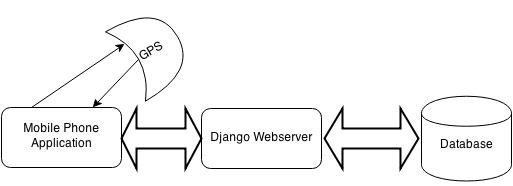
\includegraphics[width=0.7\textwidth]{images/n-tier.jpg}
  \caption{N-Tier diagram}
  \label{NTier}
\end{figure}

\subsection{Entity Relation Diagram}
\label{sec:ER}
There have been two significant iterations of the Entity Relation (ER)
diagram in this project - the first (figure \ref{ER_1}) is the final
theoretical ER model and the second is the real world implementation
with modifications and extra linking for data transfer optimisation
and changing requirements (figure \ref{ER_2}).

The first ER model collects the real-world objects in a hierarchical
structure: each \emph{Mission} has a number of \emph{Routes} that
start and end at a given \emph{Place} and each \emph{Route} is
constructed through a number of \emph{Stages}. This representation
is shown in Figure \ref{fig:route_breakdown}.

\begin{figure}[h]
  \centering
  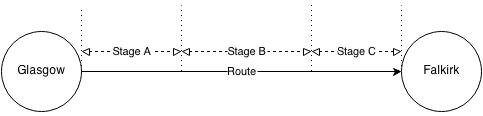
\includegraphics[width=0.8\textwidth]{images/route_breakdown.jpg}
  \caption{Breaking down a \textbf{Route} into manageable
    \textbf{Stages}}
  \label{fig:route_breakdown}
\end{figure}

It was originally intended that a user would start at a
specific \emph{Place}, Glasgow for example, and then travel along a
\emph{Route} to another \emph{Place}, Falkirk or Stirling, which
would unlock \emph{Routes} to other \emph{Places}, such as
Edinburgh. Representing this game progression of unlocking new
\emph{Routes} as you arrive at new \emph{Places} would be hard
without 
using some form of map to signify where the user can currently reach
based on the \emph{Places} they have visited. We were unable to obtain an
interactive map or discover a suitable representation that was not
ambiguous with respect to what the user was required to do to unlock a
\emph{Route}, and so the concept of travelling to \emph{Place}s to
unlock \emph{Routes} was not included in this project. However this
representation would certainly be recommended in future work as it
will provide a platform of exploration inside the game which could
encourage users. 

The \textbf{Routes Completed} and \textbf{Progress} objects in the
first ER model represent a Many to Many linking between \emph{Users}
and the \emph{Routes} and \emph{Stages} they have completed,
respectively. We note useful information here about the time taken and
completion dates which we can use to display to the user. Similarly,
the \textbf{User Achievements} table is a Many to Many linking
between the \textbf{User} and the \textbf{Achievements} table where we
store useful information relevant to when a \emph{User} was awarded an
\emph{Achievement}.

With the first theoretical ER model, managing \emph{Routes} and their 
associated \emph{Progress} along a \emph{Stage} became unwieldy from
a \emph{Session} point of view. There was no explicit linking between
these objects in a meaningful way, or indeed an efficient way to
access the relevant objects for a given session - each update to a
\emph{Session} required a lot of data transferred between the device
and the server just to know which \emph{Stage} we should update the
\emph{Progress} object of for a given \emph{User}.

Restructuring action was undertaken to introduce a manager-like object
for holding knowledge about all \emph{Progress} a user has achieved
along a given \emph{Route} and also to add a direct link between the
\emph{Session} object and the current \emph{Progress} information of
the current \emph{Route} that the \emph{User} is travelling
along. This restructuring is shown in figure \ref{ER_2}. The
manager-like object is now the \textbf{Routes Completed} object in the
production ER diagram, where we can immediately access the current
\emph{Progress} down a \emph{Route} (the \textbf{Current Journey} link
to the \textbf{Route Progress} table) and from there we can access the
\emph{Progress} along the current \emph{Stage}. 

With careful management we can also update these when we complete
either a \emph{Stage} or a \emph{Route} to allow the \emph{User} to
seamlessly move onto the next \emph{Stage} or \emph{Route} without
losing any information or incurring a large number of database
accesses by simply updating the \textbf{Current Journey} and
\textbf{Current Progress} links to the appropriate next objects. 

At the time of creating the first ER diagram, we did not know exactly
how we wanted \emph{Achievements} to work or what they would be
awarded for. After discussion it was decided that an
\emph{Achievement} should be awarded for completing a \emph{Route} in
a given time. Therefore we could create a link between an
\textbf{Achievement} and the \textbf{Route} that it is related to so
we can access \textbf{Route} information (specifically the length of the 
\emph{Route}) in an efficient manner. 

The criteria field of an \emph{Achievement} signifies the time that
the route should be created in order to be awarded this
\emph{achievement}. This field was not renamed to be a specific
\textbf{\textit{Completion Time}} field so we could keep open the
scope of what criteria an \emph{Achievement}
required. \emph{Achievements} could then be added for overall
distance/time travelled on a \emph{Route}, but this was not explored
in this project.  

\begin{figure}[p]
  \centering
  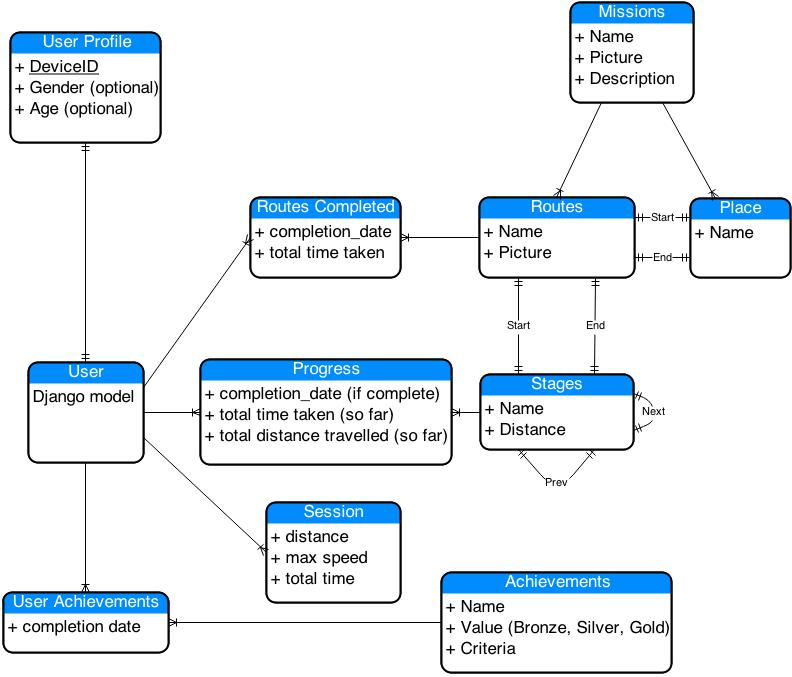
\includegraphics[width=\textwidth]{images/ER.jpg}
  \caption{ER diagram, final theoretical model}
  \label{ER_1}
\end{figure}

\begin{figure}[p]
  \centering
  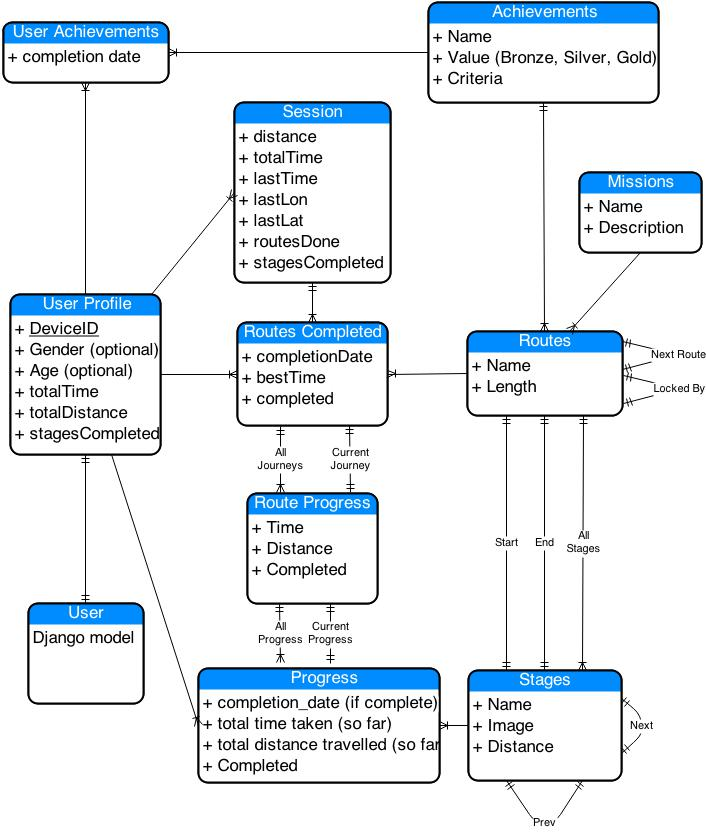
\includegraphics[width=\textwidth]{images/ER_prod.jpg}
  \caption{ER diagram, production model}
  \label{ER_2}
\end{figure}

\newpage

\subsection{Walkthrough of Workflow}
\begin{wrapfigure}{R}{0.29\textwidth}
  \vspace{-40pt}
  \centering
  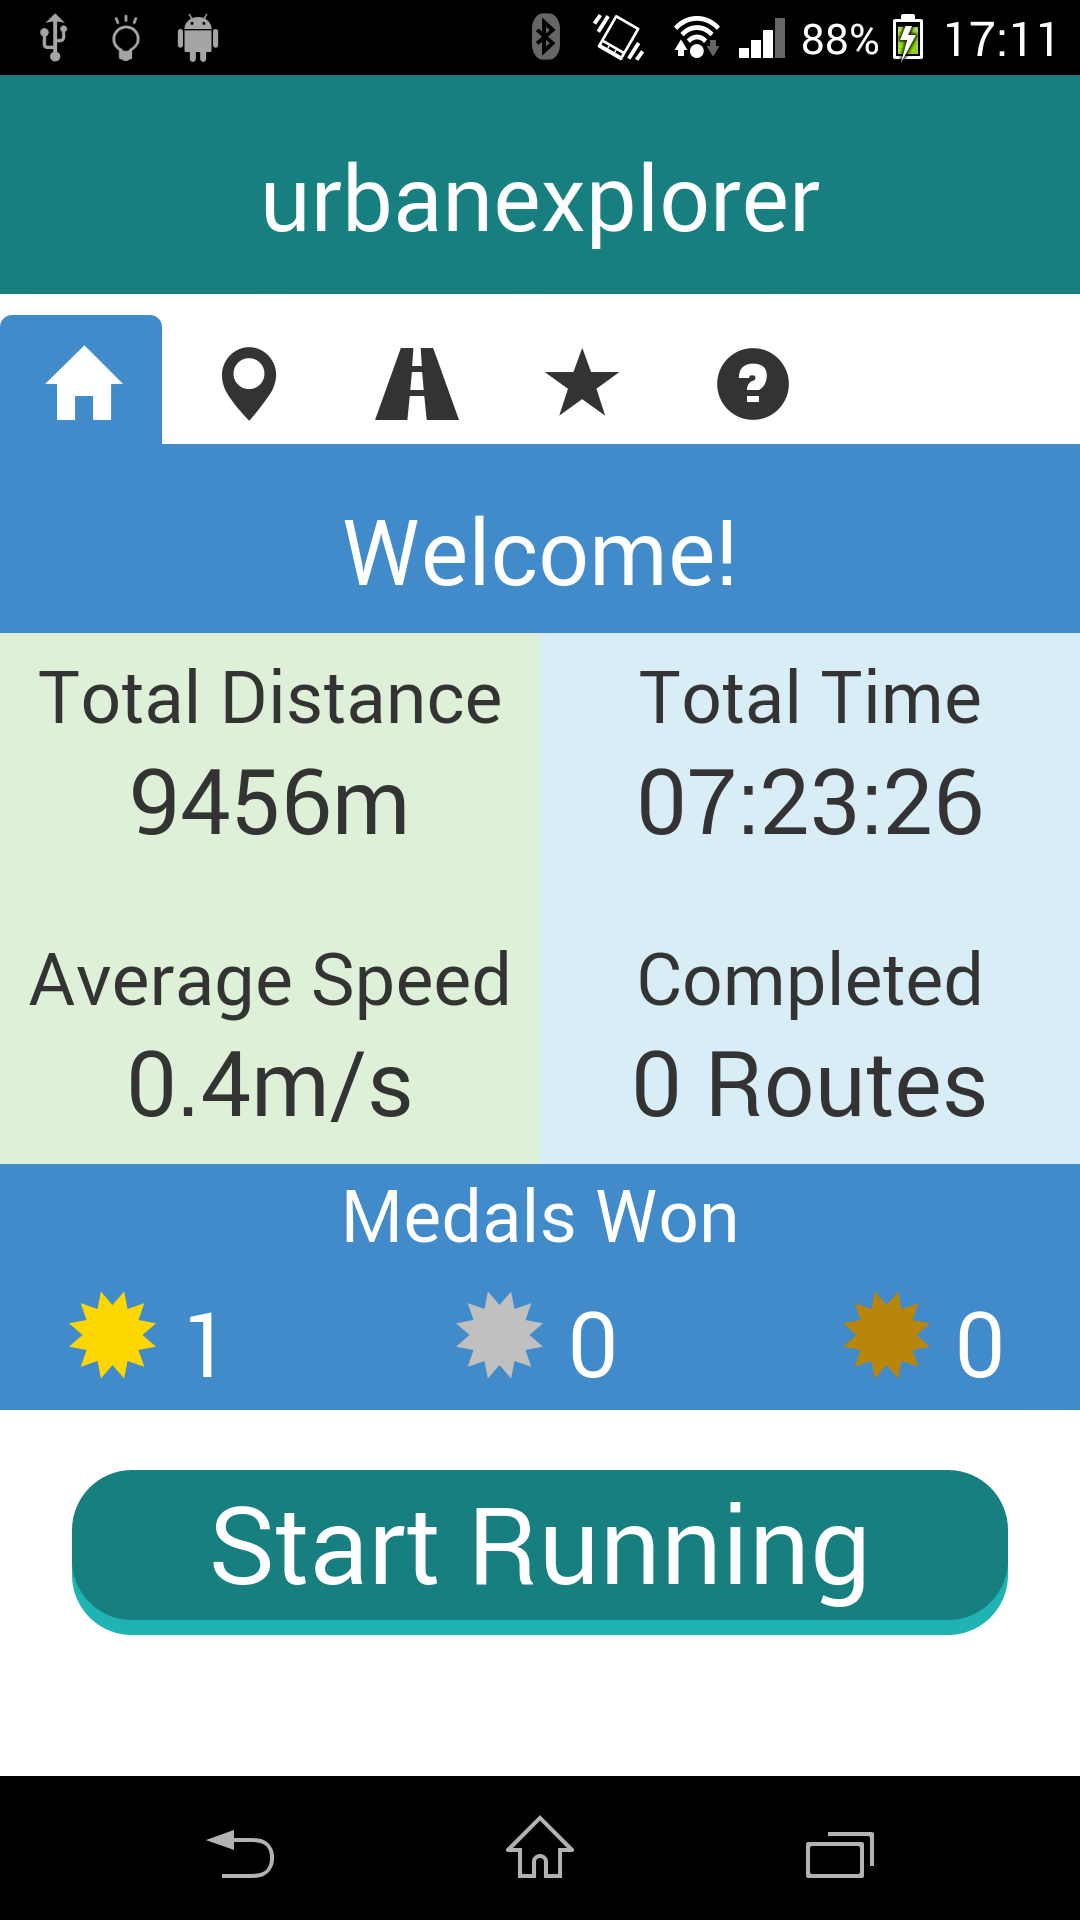
\includegraphics[width=0.29\textwidth]{images/screens/home.png}
  \vspace{-20pt}
  \caption{Home Screen}
  \vspace{-25pt}
  \label{fig:home_screen}
\end{wrapfigure}
At the beginning of the design process a workflow and set of
wireframes was drawn up to model a possible interaction scenario for 
this app\footnote{The original wireframes and walk through are listed
  in Appendix \ref{ch:original_wireframes}}. As the project evolved so
too did the workflow design. 

A tabular approach to top-level navigation, a standard Android building
block\cite{android_tabs}, was introduced to organise the different user
tasks required in the app. This can be shown in figure
\ref{fig:home_screen} where, from left to right, the tabs represent:
home screen, route selection, run/exercise session, view achievements,
and the help screen. All tabs are accessible at any time with the
exception of the center tab which can only be accessed when an
exercise session is started. Figure \ref{fig:home_screen} is the first
screen that a user will see when the app launches so we use this space
to immediately show the user statistics relating to their previous
exercise efforts.

We intend to direct the user towards starting an exercise session so
use  a large button below the statistics as a call-to-action to begin
this process. This button takes the user to the screen indicated by
the second tab: the route selection screen, shown as the first image
in Figure \ref{fig:route-exercise}. From here the user can pick a
route by tapping on it, taking the user to the center
screen in Figure \ref{fig:route-exercise} (in this example the user
has tapped on the ``Central Park Circuit'' route). 

The user can then view their current progress if they have started
this route, view what times they need to finish this route in to
achieve a medal and begin exercising by tapping the ``GO!''
button. If the user chooses to begin exercising then location
information is sought and an animation is shown to indicate that the
application is working. Once location information is obtained the user
is automatically taken to the screen shown in the last image. Here the
user is shown the picture they will achieve by completing the stage,
their current exercise statistics, the best medal they could achieve
with the time they have and their progress information. 

This path through the application quickly allows users to launch the
application, select a route and start exercising which helps to reduce
the \emph{time cost} involved in engaging with the gamification. 

\begin{figure}[h]
  \centering
  \begin{subfigure}[b]{0.3\textwidth}
    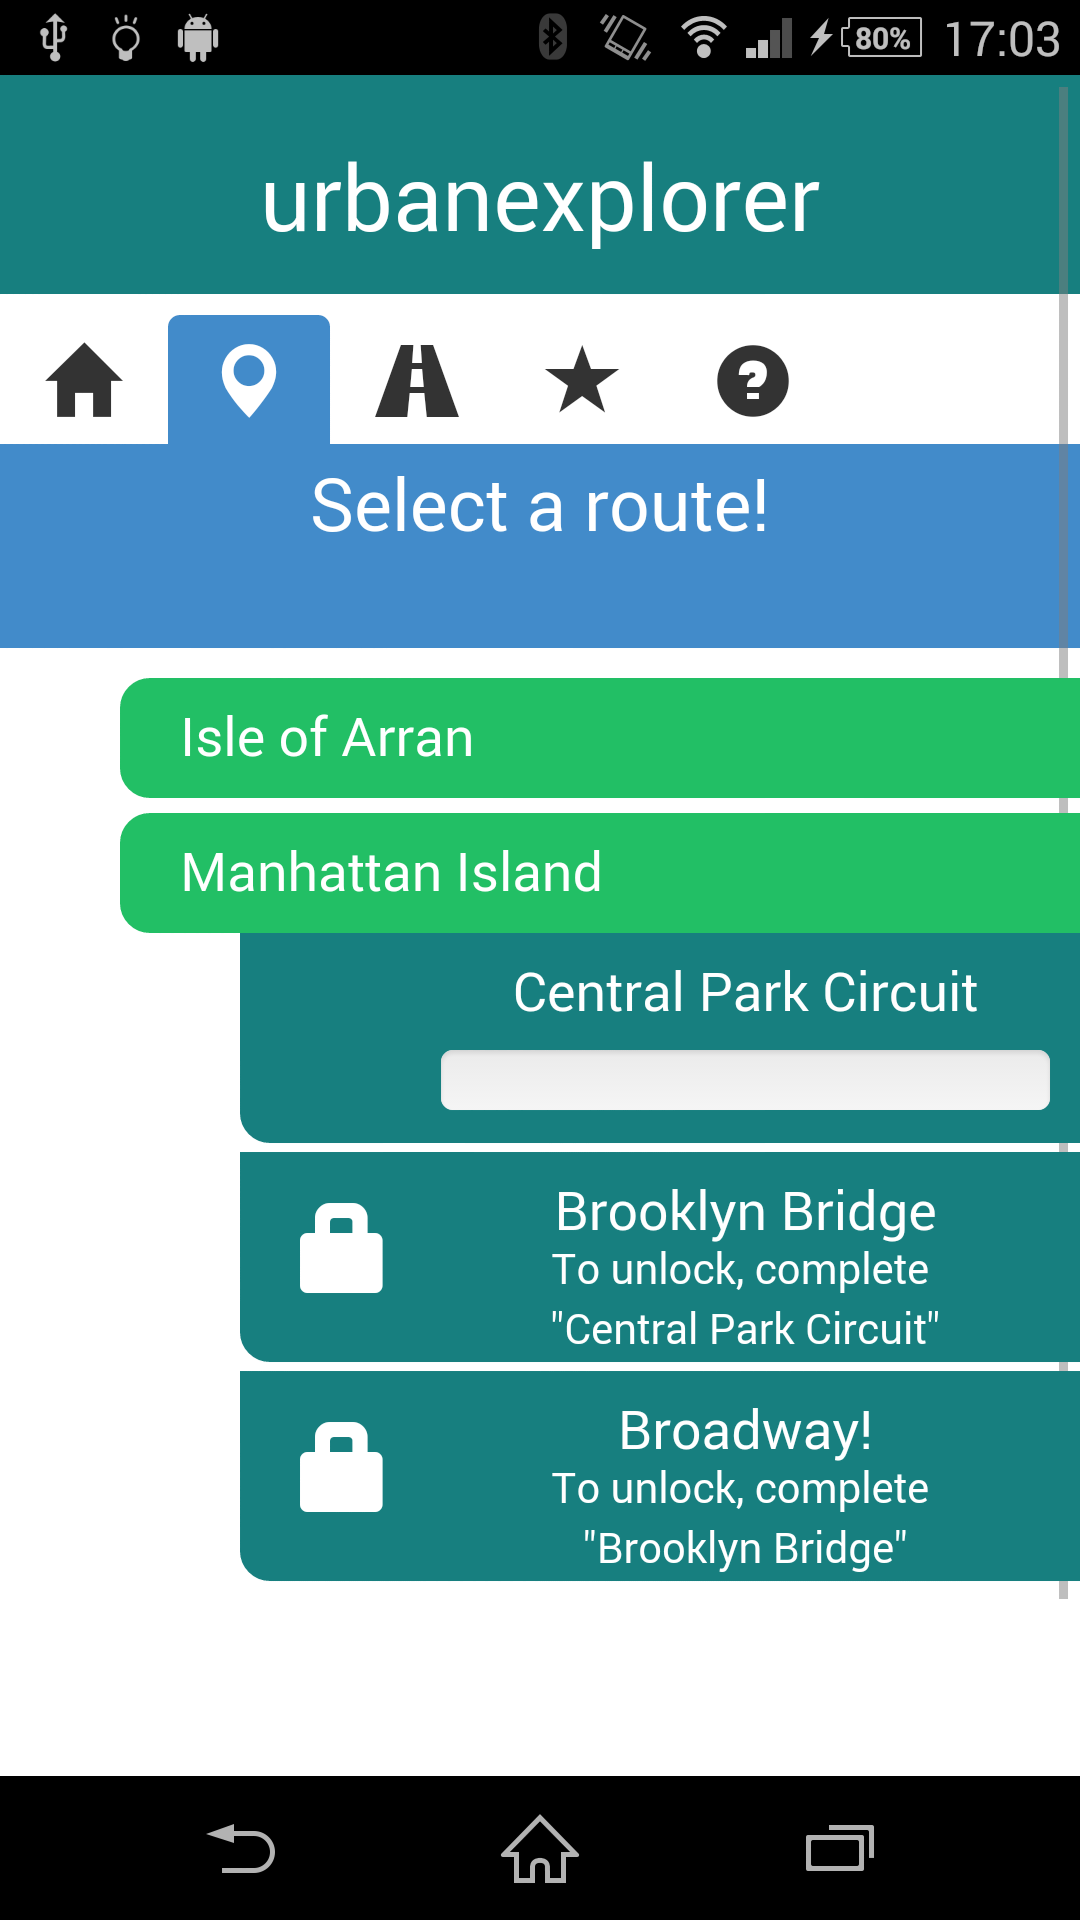
\includegraphics[width=\textwidth]{images/screens/targets.png}
  \end{subfigure}
  \hspace{0.02\textwidth}
  \begin{subfigure}[b]{0.3\textwidth}
    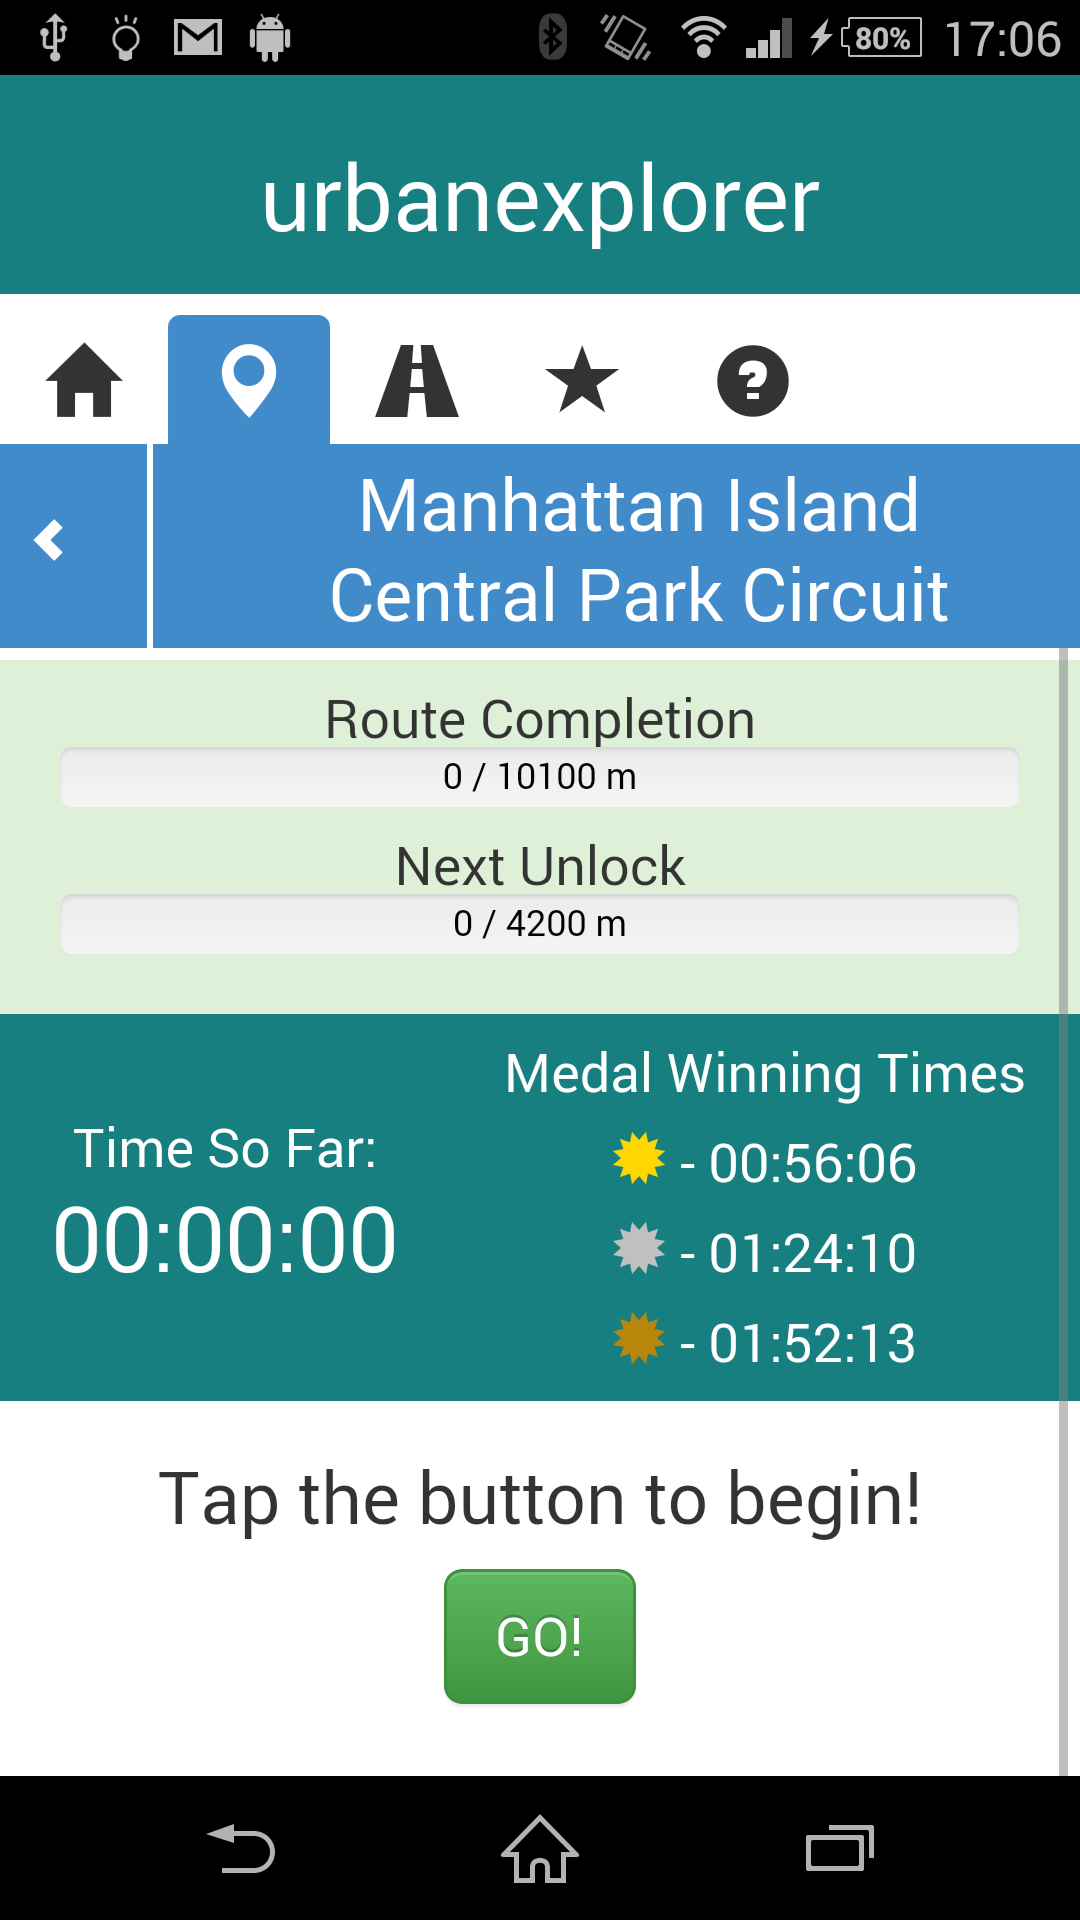
\includegraphics[width=\textwidth]{images/screens/route.png}
  \end{subfigure}
  \hspace{0.02\textwidth}
  \begin{subfigure}[b]{0.3\textwidth}
    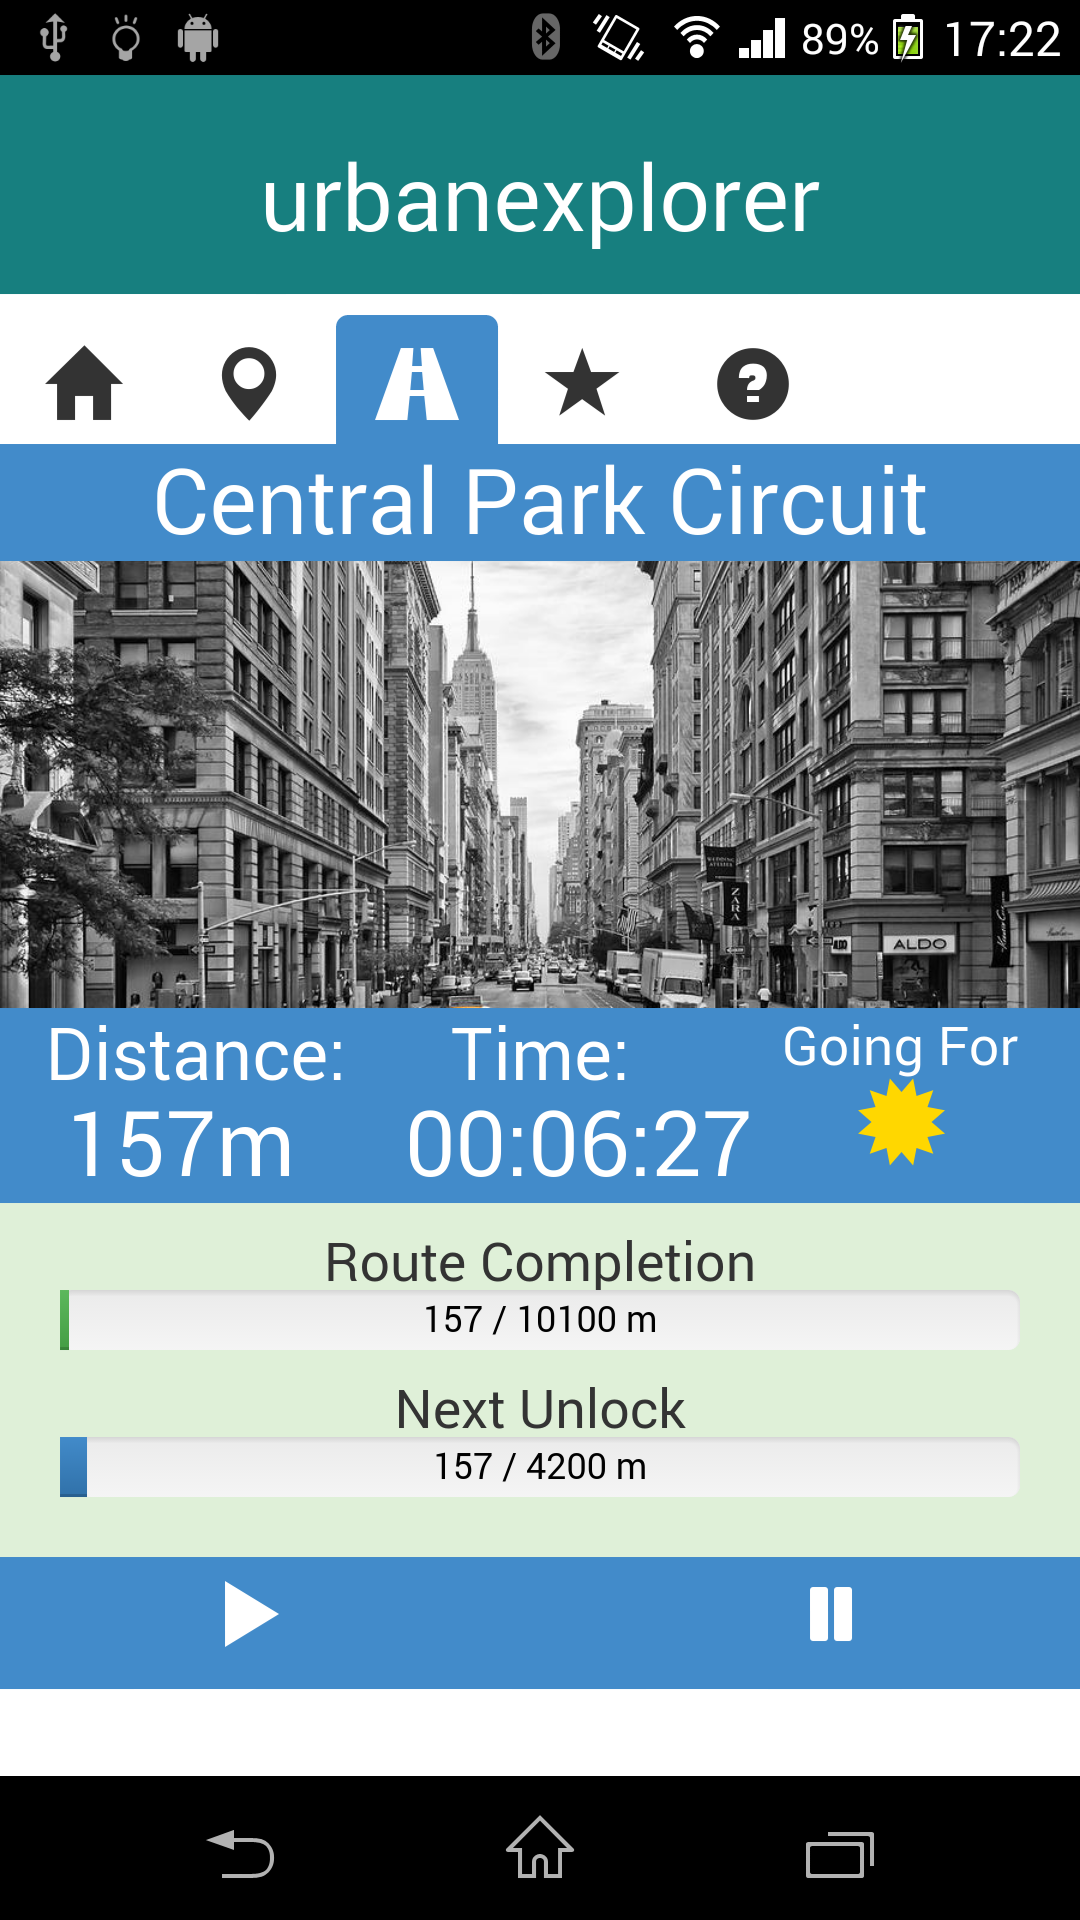
\includegraphics[width=\textwidth]{images/screens/run.png}
  \end{subfigure}
  \caption{Workflow screens for route selection through to exercising}
  \label{fig:route-exercise}
\end{figure}

\section{Notable design decisions}\label{sec:notable}
\subsection{Explicit caching}
\label{sec:explicit_caching}
As was mentioned in Section \ref{sec:specification}, the minimisation of network
traffic is of great consideration when dealing with mobile devices. We
did not want the mobile device to make repeated API calls for
resources that will not change in the short term - resources such as
what missions are available, what routes belong to what missions and
what stages belong to each route. 

The main case for this is as follows. A user may open the app for the
sole purpose of browsing all missions and their routes, and any
progress they have on these routes before they start using the app for
exercise. In an unmanaged situation the app could call the API each
time it lands on a menu to pick a mission or the routes for a mission
- if the user is browsing then they may see the same information
provided several times. 

If we remove data transfer from the equation all together and focus
solely on the user experience then caching will give a better user
experience in terms of loading speed. Since caching means we do not
have to hit the API each time we want to see something we have seen
before, we can load selection menus faster. 

Note that only data endpoints that are unlikely to change in the short
term or those that cannot feasibly change under certain circumstances
are cached. The ``progress'' endpoint which provides the data about a
users progress along given stages will not change if the user does not
initiate an exercise session - the user has not made any more progress
so it could not have changed.

These caching services are used as singleton-like facilities in the
application to ensure consistent data throughout the application, an
update to this data will be reflected throughout the entire
application. 

\subsection{Promise Based Module Interfaces}
Each module that has been created for managing either a specific set
of objects(routes, missions or the user object) has been defined
with a common interface. This common interface brings a regular
and well defined way of interacting with these modules, especially if
they utilise explicit caching (section \ref{sec:explicit_caching}) or
execute asynchronous methods.

There are two ways that this consistent interface could be
implemented: a function callback explicitly provided as an argument to
the module function call; or by using promises.

Function callbacks passed as parameters are a common JavaScript
paradigm. They are used in the PhoneGap framework to interface with
the device\cite{phonegap_currentpos}. A frequent problem with function
callbacks is what is colloquially known as ``callback hell''
\cite{callback_hell} where nested anonymous functions are used to
bring an order of execution to asynchronous tasks. This can become
unmanageable and hard to maintain in larger projects but can be
overcome with good software development procedures. An example of how
the callback approach works is show in Figure \ref{fig:callbacks}.

\begin{figure}[h]
\begin{verbatim}
function async(callback){
  // Do something with the args asynchronously.
  // Then explicitly call the callback function.
  callback(data);
}

function callback(data){
  // do something with the data returned from the asynchronous task.
  console.log(data);
}

// Invoke the asynchronous function and process the returned data.
async(callback);
\end{verbatim}
\caption{Callback approach to asynchronicity}
\label{fig:callbacks}
\end{figure}

The biggest problem for us is the framework we are using - AngularJS
only knows about events that happen in its own scope. This means that
when we invoke the callback function with the data from a module, the
data will be updated in the controller but AngularJS does not know to
update any reflections of this data in the DOM or elsewhere. There are
ways to notify the framework that it should run an update (known as a
digest cycle)\cite{angularjs_apply} but if we invoke this when a
digest cycle is currently in progress then the framework throws an
error and drops the request.

Another option is to use the AngularJS wrapping for the standard
``setTimeout'' function with a delay of zero. The ``setTimeout''
function executes a callback function after a certain time
period\cite{setTimeout}. While this may seem
frivolous, a subtlety of this wrapping avoids the digest cycle clash
of the above problem. The AngularJS wrapper ``\$timeout'' will invoke
the function passed to it after the delay expires, but importantly
will cause a natural digest cycle to occur. So if this is called using
a delay of zero then we make AngularJS update without risk of the
framework erroring. This is the method that we use inside the ``core''
set of modules that wrap the PhoneGap device API
methods\cite{wrappingPhonegap} as they use callbacks as their own
notification method. Wrapping using ``\$timeout'' can be shown in
figure \ref{fig:timeout} (note this is an example that is stripped of
the necessary declarations to work in the framework, it is intended as
an example only).

\begin{figure}[h]
\begin{verbatim}
\\ PhoneGap function to get the users location,
\\ success and failure are two callback functions.
\\ Note the similarity to the previous example.
geolocation.getCurrentPosition(callback)

\\ This is defined in our controller or other module.
function success(data){
  \\ Call the $timeout function with delay of zero to safely invoke
  \\ on next digest.
  $timeout(function(){
    \\ do something with the location data
    \\ AngularJS knows about this update.
  }, 0);
}

\\ Invoke request for location information.
geolocation.getCurrentPosition(success);
\end{verbatim}
\caption{Using ``\$timeout'' to wrap PhoneGap API}
\label{fig:timeout}
\end{figure}

Internally within modules the ``\$timeout'' method is used for
notifying the framework of necessary change as PhoneGap uses callbacks
as its own notification method. Callbacks could also be used for
inter-module communication but would require each callback function to
use the ``\$timeout'' method if any asynchronicity occurs. Since we
want to develop a consistent interface between all modules this is not
appropriate: we need to know when we should and should not require a
call to ``\$timeout'' when we write the callback function, and this
can be different between modules. 

The \emph{\$timeout} method is also
not elegant, read colloquially as a ``hack'', and it is not obvious to
a new developer why this function should even be called. In some cases
it is the only safe approach but for all others it would be bad
software practice to use this approach when other better solutions
exist. 

We can remove all these complexities by using
promises\footnote{Promises -
  \url{https://developer.mozilla.org/en-US/docs/Web/JavaScript/Reference/Global_Objects/Promise}}
. A promise allows us to manage deferred (asynchronous) callbacks and
synchronous callbacks in the same way. Helpfully the AngularJS
framework has promises integrated in with the digest cycle management
so we do not need to be concerned with this issue any more. 

Promises and callbacks are theoretically similar as both provide a
function to be called once something has occurred however promises do
not suffer from the ``callback hell'' anti-pattern that callbacks
alone do due to a flow control change.
Kris Kowal, the creator of the promise library ``Q'' that
AngularJS bases its promise library ``\$q'' on, defines the flow
control change as follows:
\begin{quote}
The callback approach is called an ``inversion of control''. A function
that accepts a callback instead of a return value is saying, ``Don’t
call me, I’ll call you.''. Promises un-invert the inversion, cleanly
separating the input arguments from control flow arguments.\cite{kriskowalq}
\end{quote}

A function that uses promises to notify success or failure immediately
returns a promise object. This is different to the callback approach
as the program is allowed to continue to execute as the function
immediately returns, unlike the callback approach which blocks for the
response, and the function to handle the response is invoked when a
response is ready. These response handlers are attached to the promise
object by calling the ``then'' method of the promise, and these are
called when the promise resolves. This can be shown in Figure
\ref{fig:promises}. 

\begin{figure}[h]
\begin{verbatim}
// This could be in another module, but doesn't need to be.
function promiseFn(){
  \\ Create a new promise
  var deferred = $q.defer();
  var data = {}; \\ Data from (a)synchronous task stored in here.  

  \\ Something asynchronous or sychonous here. Once it's completed...
  \\ Resolve the promise
  deferred.resolve(data);

  \\ return the promise
  return deferred.promise;
}

function processData(data){ ... //Do something with data }

// Call function and process the data it returns.
promiseFn()
  .then(processData);
\end{verbatim}
\caption{Using Promises in AngularJS}
\label{fig:promises}
\end{figure}

Although promises are intended for use when there is asynchronous
behaviour, they can also be used in synchronous situations. The exact
user-perceived behaviour would also occur if the asynchronous task was
made synchronous in figure \ref{fig:promises}. The functions passed to
the ``then'' method of a promise will be called when the promise is in
a state of being resolved, so they can be added before or after the
promise is resolved and they will be called in both cases.

This then provides us a method that allows a consistent interface that
integrates well with AngularJS. It is worth noting that the
``\$timeout'' method is used with modules that interface with any of
the PhoneGap device API methods that are asynchronous. As is discussed
previously, this is to notify AngularJS that a promise has changed
state in a situation that it does not know about. So although promises
solve most of our problems, they do not completely solve all of them.

\subsection{Exercise Session Management}
\label{sec:session_mgmt}
Due to the environmental implications brought on by GPS, we may not be
able to identify their location. The user should not
be penalised for this as it is outwith their control and is not a
direct error on their part. Something as simple as running through a
tunnel could initiate the loss of signal. 

To counter this, the exercise session is designed in such a way as to
not penalise or disadvantage the user if they should not be able to
obtain location information. 

When a user decides to exercise, a new session is created through the
API. The users device is then given a unique ID for that session that
only they have a knowledge of (in the first iteration of this
implementation this ID is a direct mapping to the ID of the object in
the database, but in a future version this could be something more
obscure). Only this user can update this session and it can only be
updated if you know the unique ID for that session. 

This ID is saved on the users device for the duration that the user
wants the session to be active and is deleted when the user either
closes the app or explicitly ends the session. We can then update the
session successfully when we have a GPS location and are ready to
update, while indirectly ``ending'' the session when we delete the
unique ID.

If the user cannot obtain location information then the device will
retain the unique ID for the session and will update as soon as it can
obtain location information. This is explored further in section
\ref{sec:location_mgmt}.

This does guarantee that the user will gain all distance they should
be awarded. If the user starts an exercise session but cannot then
obtain location information and either exits the app or ends the
exercise session then the user will not be credited for the distance
they travel. This is a situation we cannot control and so we can
accept that this is a limitation of the implementation.

When a session is created we need to tell the server what route we
intend to travel down and where we currently are (in terms of our
longitude and latitude). To update a session, we only need to provide
a timestamp, longitude and latitude positioning and the session
ID. On receipt of a successful update the server will update what
stage a user is on, automatically moving the user onto the next stage
on a route when they complete their current stage. 

Only the last known location (set of longitude and latitude
coordinates) and the time that the user was at those coordinates are
kept in the server. We only need the last location 
to work out distance a user has travelled since the last update. 

We have two options when a user completes a stage: we can either
accumulate the excess distance they travel and allow the user to
``spend'' this distance on whatever route they like when they finish;
or automatically advance the user onto the next sensible route. 

The latter option was chosen for this implementation as it is the most
immersive option of the two. From a game perspective, the first option
does not allow the user to fully engage in the game at the time they
are playing as no further rewards are accumulated when distance is not
being incremented while the second allows the user to continue
progressing seamlessly. 

\subsection{Location Management}
\label{sec:location_mgmt}
PhoneGap exposes two main ways to obtain location information, either
by requesting where the device is at this exact moment in
time\cite{phonegap_currentpos} or by requesting to be updated at a
discrete time interval when the device position
updates\cite{phonegap_watchpos}. 

The original intention was to use the first method to manually control
the time between requesting new location information so that if a
request fails we can immediately send a request again. This method was
dropped after closer inspection of the plugin that provides these
services and research into how the Android Location Manager handles
location data.

The plugin that provides the location data links directly to the
Android Location Manager as expected. This location manager handles
all requests for location data from all applications running on the
device. The second method of obtaining location information registers
a watcher with this Location Manager and allows the Location Manager
to handle the polling for coordinates. If location information cannot
be obtained then we rely on the Location Manager to deal with
retrying. 

As much as we may wish to immediately retry searching for coordinates
with the intention of keeping accurate distance information for a
user, this may have negative repercussions. Obtaining accurate
location information is a costly operation requiring 50-200mA for each set
of coordinates, more when there is no recent location
information\cite{android_power}. It is the fourth most power intensive
operation an app developer can invoke, as shown in figure
\ref{fig:power} \cite{android_efficiencySlides}.

\begin{figure}[h]
  \centering
  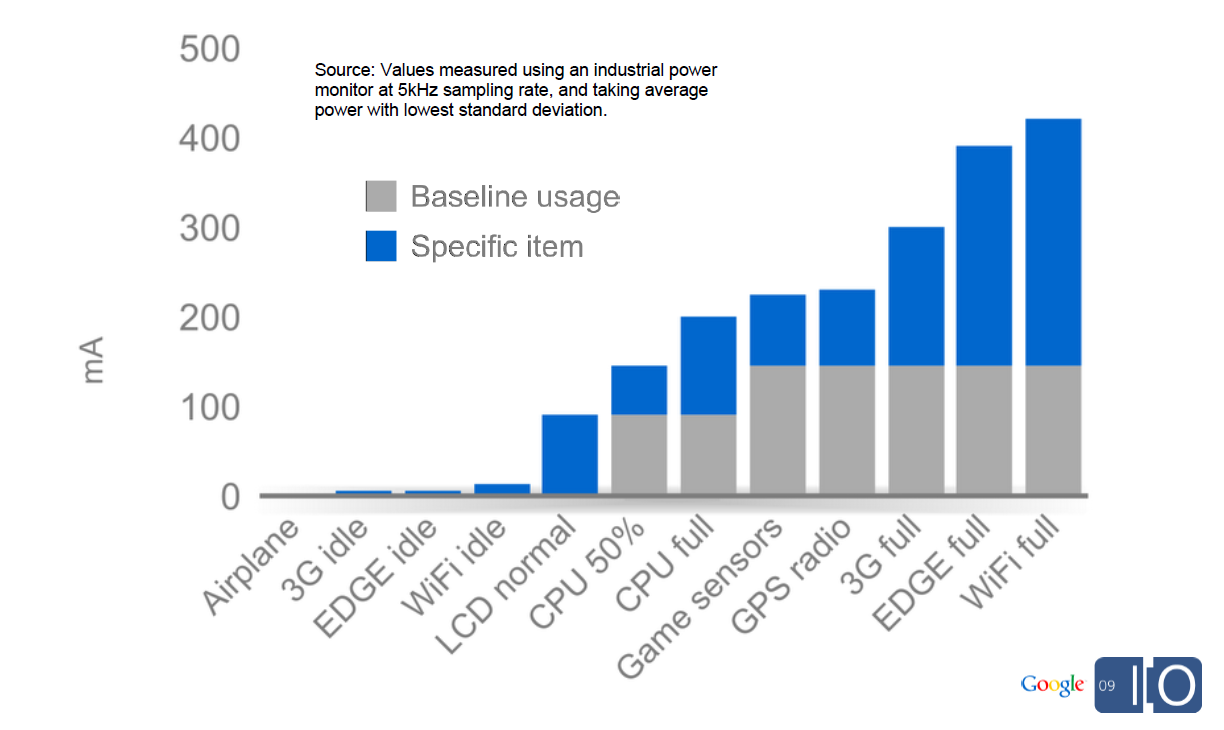
\includegraphics[width=\textwidth]{images/power.png}
  \caption{Power Consumption of sensors on Android Devices \cite{android_efficiencySlides}}
  \label{fig:power}
\end{figure}

In the situation where we will not be able to obtain location
information, when a user enters a tunnel for example, it would be
unnecessary to repeatedly ask for location information. The only
outcome in this scenario is a faster drain on the users battery which
could lead users to have a negative experience with the app. So even
though we are leading with the best of intentions it is not the right
decision to make. Due to the round trip time required to notify the
server of new location information and the relatively short distances
users can travel, it was decided that the provided interval of one
update a minute was sufficient to ensure a balance between power and
accuracy. 

Polling for location information once a minute does suffer from one
drawback we will define as the ``Cul-de-sac Effect''. The Cul-de-sac
Effect arises between two location updates where the user travels a
significant distance between these two updates but these location
updates occur close to one another, resulting in a much smaller
perceived distance. This effect arises when we reduce update
frequency to increase power conservation and can be shown in figure 
\ref{fig:cul-de-sac} where we assume all location updates (noted as
``GPS Location'') occur consistently at a discrete time interval. 

\begin{figure}[h]
  \centering
  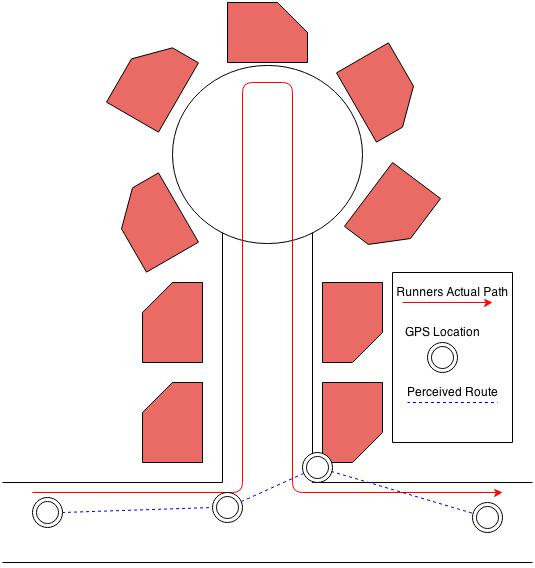
\includegraphics[width=0.7\textwidth]{images/cul-de-sac.jpg}
  \caption{Example of the ``Cul-de-sac Effect''}
  \label{fig:cul-de-sac}
\end{figure}

In the contrived example shown in figure \ref{fig:cul-de-sac} we have
no evidence that the user has travelled into the cul-de-sac, as we
base our distance calculations solely from the location information,
and so we cannot award them the distance they have actually
travelled. Therefore the user is unnecessarily penalised through the
unfortunate circumstances of timing and their route choice. 

The ``Cul-de-sac'' effect is a domain-specific example of
aliasing. Aliasing occurs when one samples a signal at a frequency
that is far lower than the frequency of the original signal and
produces an alternate signal that is an incorrect representation of
the original one, but is indistinguishable to the original one with
respect to the sampling points. This can be shown in Figure
\ref{fig:ailising} where the red and blue signals are
indistinguishable with respect to the black sampling points.

\begin{figure}
  \centering
  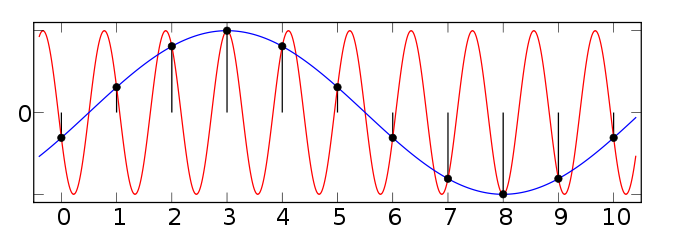
\includegraphics[width=\textwidth]{images/aliasing.png}
  \caption{Aliasing of two signals. \cite{ailising}}
  \label{fig:ailising}
\end{figure} 

In Section \ref{sec:distance_ver}, we will define the maximum speed we
allow users to travel at to be $\text{6}m/s$. In the worst case of this
effect the users device will return location information that informs
us the user has moved no distance (the coordinates are exactly the
same). If we assume that we receive the location updates exactly once
a minute then the worst case distance that the user could lose due to
this effect is $\text{360}m$ . This is a considerable distance and the
unacknowledged effort could have a large negative effect on the
user. Further work is required to analyse this effect to find the best
update frequency interval with respect to this effect and power
consumption. 


\subsection{Distance Verification}
\label{sec:distance_ver}
To create an exercise session a set of longitude and latitude
coordinates are required. By enforcing this requirement we are always
able to know where a user was last and then work out the distance they
have travelled when new coordinates are provided. 

Converting two pairs of longitude and latitude coordinates to a
distance in kilometers is done through the Haversine
function\cite{haversine} with a Python module of the same
name\cite{python_haversine}. The Haversine function converts these
coordinates to a distance with respect to the curvature of the Earth,
giving us greater accuracy in our distance calculations.

We send the coordinates to the server and compute the distance there
instead of on the mobile device in the interests of verifying that
the distance is correct. If a user only sends a distance and not a
set of coordinates then we have no mechanism of determining if that
distance is valid or not, whereas if we are given coordinates then we
have a reference point to compare to (since we retain the last known
coordinates). It can be argued that even this is not enough to fully
guarantee that the location information provided is honest but there
is little we can do to ensure honesty in this case. 

We can however limit the distance we update by based upon whether or
not that distance is physically possible. A timestamp is required when
updating with a set of coordinates and so we can compute the speed the
user was travelling at over the time period since their last
update. If this speed is greater than a fixed maximum travel speed
then action is taken to reduce the distance to the maximum distance
the user could have travelled in this interval. This process is shown
in Figure \ref{fig:distance_limit}.

\begin{figure}[h]
\begin{equation*}
  distance = haversine(coordinates_{old}, coordinates_{new})
\end{equation*}
\begin{equation*}
  time = timestamp_{new} - timestamp_{old}
\end{equation*}
\begin{equation*}
  speed_{actual} = \frac{distance}{time}
\end{equation*}
\begin{equation*}
  distance = \left\{
  \begin{array}{l l}
    distance & \text{if $speed_{actual} \leq speed_{max}$} \\
    speed_{max} \times time & \text{if $speed_{actual} > speed_{max} $}
  \end{array}
  \right\}
\end{equation*}
\caption{Limiting the distance a user can travel based on a maximum speed.}
\label{fig:distance_limit}
\end{figure}

The maximum speed we allow users to travel at is $\text{6}m/s$ as this
accommodates for walking, running and sprinting.

This action to limit the distance travelled based on the time period
will help to defend against cheating but will not negatively impact
users who cannot obtain location information for an arbitrary time
period. A user could still upload bogus coordinates to the server but
this limiting will help to reduce the effectiveness of their
cheating. This would also require the user to know the URL schema of
our server, which is not publicised. The gain they would receive is
not proportional to the time they would spend on this cheating attempt
and so it is unlikely that anyone should try this.



